\documentclass[main.tex]{subfiles}

\begin{document}
\chapter{Modern machine learning algorithms and their uses}
\label{chapter:ml}
\section{Rise of machine learning in HEP}
    In high energy physics, where analyses
    depend on making use of large computing clusters
    and international grid efforts \cite{WLCG}, advancements
    in technology and more efficient methods are
    required to keep up with the needs of the
    experimental and theoretical communities.
    However, the computational resources needed
    are at risk of outpacing the growth in these research
    areas \cite{Bothmann:2022thx}, especially with
    HL-LHC projected to begin operating at the end
    of this decade \cite{ZurbanoFernandez:2020cco}.
    Therefore new techniques and
    algorithms from machine learning 
    have been adopted to augment the ongoing efforts
    in high energy physics. Machine
    learning is a category of artificial intelligence
    concerned with the design of algorithms that
    automates learning from data.
    By now, machine learning is ubiquitous in
    particle physics analysis, from collection
    of data from experiments, all the way to novel
    applications on the theory side.

    Around the turn of the last decade the culmination
    of advancement in hardware and training algorithms
    led to an explosion in research in the
    machine learning community, specifically in the
    utilisation of very large neural networks. The accuracy
    of these deep neural networks greatly outperformed the
    previous state of the art \cite{NIPS2012_c399862d,russakovsky2015imagenet} and
    lead to the widespread use of neural networks across
    a range of tasks \cite{Schmidhuber_2015}.
    This led to the rise of programming
    frameworks such as scikit-learn \cite{scikit-learn},
    TensorFlow \cite{tensorflow2015-whitepaper},
    PyTorch \cite{paszke2019pytorch},
    and XGBoost \cite{Chen:2016:XST:2939672.2939785}
    to name a few which implement neural networks, alongside
    other mainstay algorithms such as decisions trees.
    These algorithms are now extremely commonplace
    in many domains, including in particle physics. 

    Collisions at the LHC can produce hundreds of
    particles with complex final-state configurations.
    This leads to the design of the ATLAS and CMS experiments
    to contain of the order 100 million detection elements
    in an attempt to disentangle these events. With these large
    arrays, petabytes of data are recorded every year
    across all LHC experiments.
    This presents a practical challenge for data
    collection where machine learning has could provide a solution.
    Indeed, boosted decision trees have been use
    to enhance triggers \cite{CMS:2020cmk} to accept or
    reject data before being saved to disk.
    % At the LHCb
    % experiment, 70\% of all data retained have had
    % some contact with machine learning algorithms \cite{LHCb:2014set}.

    In view of the upgrades at the LHC and the upcoming
    HL-LHC providing unprecedented integrated luminosity,
    it is important that the generation of simulated samples
    is accelerated. This prompted the explosion of research
    in machine learning applications on the theory side.
    Studies have been carried out on many stages of the event
    generation process.
    To name just a few examples of active research areas:
    phase-space sampling \cite{Bendavid:2017zhk,Klimek:2018mza,Bothmann:2020ywa,Verheyen:2020bjw,Gao:2020vdv},
    matrix element modelling \cite{Bishara:2019iwh,Badger:2020uow,Aylett-Bullock:2021hmo,Maitre:2021uaa,Badger:2022hwf},
    hadronisation modelling \cite{Biro:2021zgm,Ilten:2022jfm,Ghosh:2022zdz},
    and end-to-end event generation \cite{Gao:2020zvv,DiSipio:2019imz,Butter:2019cae,Butter:2021csz,ArjonaMartinez:2019ahl}.
    For a more complete overview of active research,
    a living review that is archiving advancements in the
    field is available at Ref. \cite{Feickert:2021ajf}.
    For more traditional reviews, see Refs.
    \cite{Guest:2018yhq,Radovic:2018dip,Butter:2022rso}.

    The research carried out in these areas have shown
    promising results but a challenge that remains
    is to interface these novel machine learning methods
    to existing event generators for real-world use.
    There is scepticism regarding the use of machine learning
    algorithms in production due to their lack of interpretability \cite{Grojean:2022mef},
    as well as their use as black-boxes which precludes predictability \cite{Schwartz:2022njo}.
    Along similar lines, the quantification of the uncertainties
    associated with these algorithms are not well defined \cite{Chen:2022pzc}.

    In this chapter we give an overview of neural
    networks: how they are constructed, how
    they are trained, and how their parameters are optimised.
    We will then proceed to discuss their
    application to modelling matrix
    elements with a review of the current
    state of the art methods.

\section{Neural networks}
    Neural networks are a machine learning algorithm
    inspired vaguely by the structure of the human brain.
    That is to say they are an interconnected network
    of neurons used for analysing data. Here, we will
    introduce the densely-connected neural network
    which will be the main workhorse algorithm used
    in this thesis, and frame the discussion around a
    regression task. Namely, how to use sampled training data
    from a target function $g(\mathbf{x})$ to create a surrogate
    model with a neural network algorithm.

    In a machine learning context, the fitting of a
    model to data is termed training the model.
    Once the model is fitted, it is customary to use
    an unbiased dataset that is distinct from the training set, the test set,
    to evaluate the final model performance.

\subsection{Model of a neuron}
    In this context, a neuron is described by
    \begin{equation}\label{eqn:neuron}
        y = \phi(\mathbf{w}^{T}\mathbf{x} + b) = \phi_{\theta}(\mathbf{x})
    \end{equation}
    where the model inputs, $\mathbf{x}$, are multiplied
    by the model weights, $\mathbf{w}$, before being summed
    with a bias term, $b$. Collectively, the model weights
    and biases are the model parameters, $\theta$.
    This combination of terms is then modified
    by an activation function, $\phi$, which is carefully
    chosen to perform a non-linear transformation. The
    notation $\phi_{\theta}$ represents an activation function
    acting on $\mathbf{x}$ which has been combined with parameters $\theta$.
    A neuron is illustrated in Figure~\ref{fig:neuron}.
    
    \begin{figure}
        \ctikzfig{img/ml/neuron}
        \caption{A schematic diagram of a neuron. The model inputs
        $\mathbf{x}$ and weights $\mathbf{w}$ are vectors, whereas
        the bias $b$ is a scalar. The weighted inputs are summed with
        the bias before passing through an activation function
        to give the scalar output $y$.}
        \label{fig:neuron}
    \end{figure}
    
    Some of the more well-known activation functions are
    the sigmoid function, hyperbolic tangent, and the rectified linear unit (ReLU) \cite{Nair2010RectifiedLU}.
    A less familiar class of activation functions are the
    sigmoid linear units (SiLU) \cite{Hendrycks2016BridgingNA},
    of which swish \cite{DBLP:journals/corr/abs-1710-05941} is an example.
    The functional forms of these
    functions and their gradients are summarised in Table~\ref{table:activation_functions}.
    There is no single activation function that is the best
    for any given task, and it is common practice to choose activation
    functions on a case-by-case basis.

    \begin{table}
        \centering
        \begin{tabular}{lll}
            \toprule
            Activation & Functional form & Gradient \\
            \midrule
            Linear & $f(x) = x$ & $f'(x) = 1$ \\
            \midrule
            Sigmoid & $f(x) = \dfrac{1}{1+e^{-x}}$ & $f'(x) = f(x)(1-f(x))$ \\
            \midrule
            Tanh & $f(x) = \tanh(x)$ & $f'(x) = 1 - f(x)^{2}$ \\
            \midrule
            ReLU & $f(x) = \begin{cases} 0 \, , \quad \mathrm{for} \quad x \leq 0 \\ x \, , \quad \mathrm{for} \quad x > 0 \end{cases}$ & $f'(x) = \begin{cases} 0 \, , \quad \mathrm{for} \quad x \leq 0 \\ 1 \, , \quad \mathrm{for} \quad x > 0 \end{cases}$ \tablefootnote{The gradient of ReLU is not defined at $x=0$ but for a numerical implementation, defining it to be 0 at this point is sufficient.} \\
            \midrule
            swish & $f(x) = \dfrac{x}{1+e^{-x}}$ & $f'(x) = \dfrac{1}{x}f(x) \left[(1+x) - f(x)\right]$ \\
            \bottomrule
        \end{tabular}
        \caption{Functional forms of common activation functions and their gradients.}
        \label{table:activation_functions}
    \end{table}

\subsection{Densely-connected neural networks}
    In order to build a neural network, the neurons
    have to be connected in some fashion. Perhaps
    the most straightforward method is to create
    layers of neurons, and then connect every neuron
    in a layer with every neuron in neighbouring layers.
    This is illustrated in Figure~\ref{fig:nn_example}.
    Such a configuration is called a fully-connected,
    or densely-connected neural network. The constituents
    of this network structure are: the input layer where
    model inputs enter; hidden layers, where the bulk of
    model parameters live; and the
    output layer which outputs the model prediction(s).
    The training data only provides concrete, desired
    outputs for the overall model, and does not specify
    anything about the layers preceding, hence the term hidden.
    The neural network is free to change the parameters
    in these hidden layers to best approximate the target function
    $g(\mathbf{x})$.
    Output layers are functionally the same as hidden
    layers, except that their outputs are taken as the
    model prediction and so can be compared with the truth
    value.
    
    \begin{figure}
        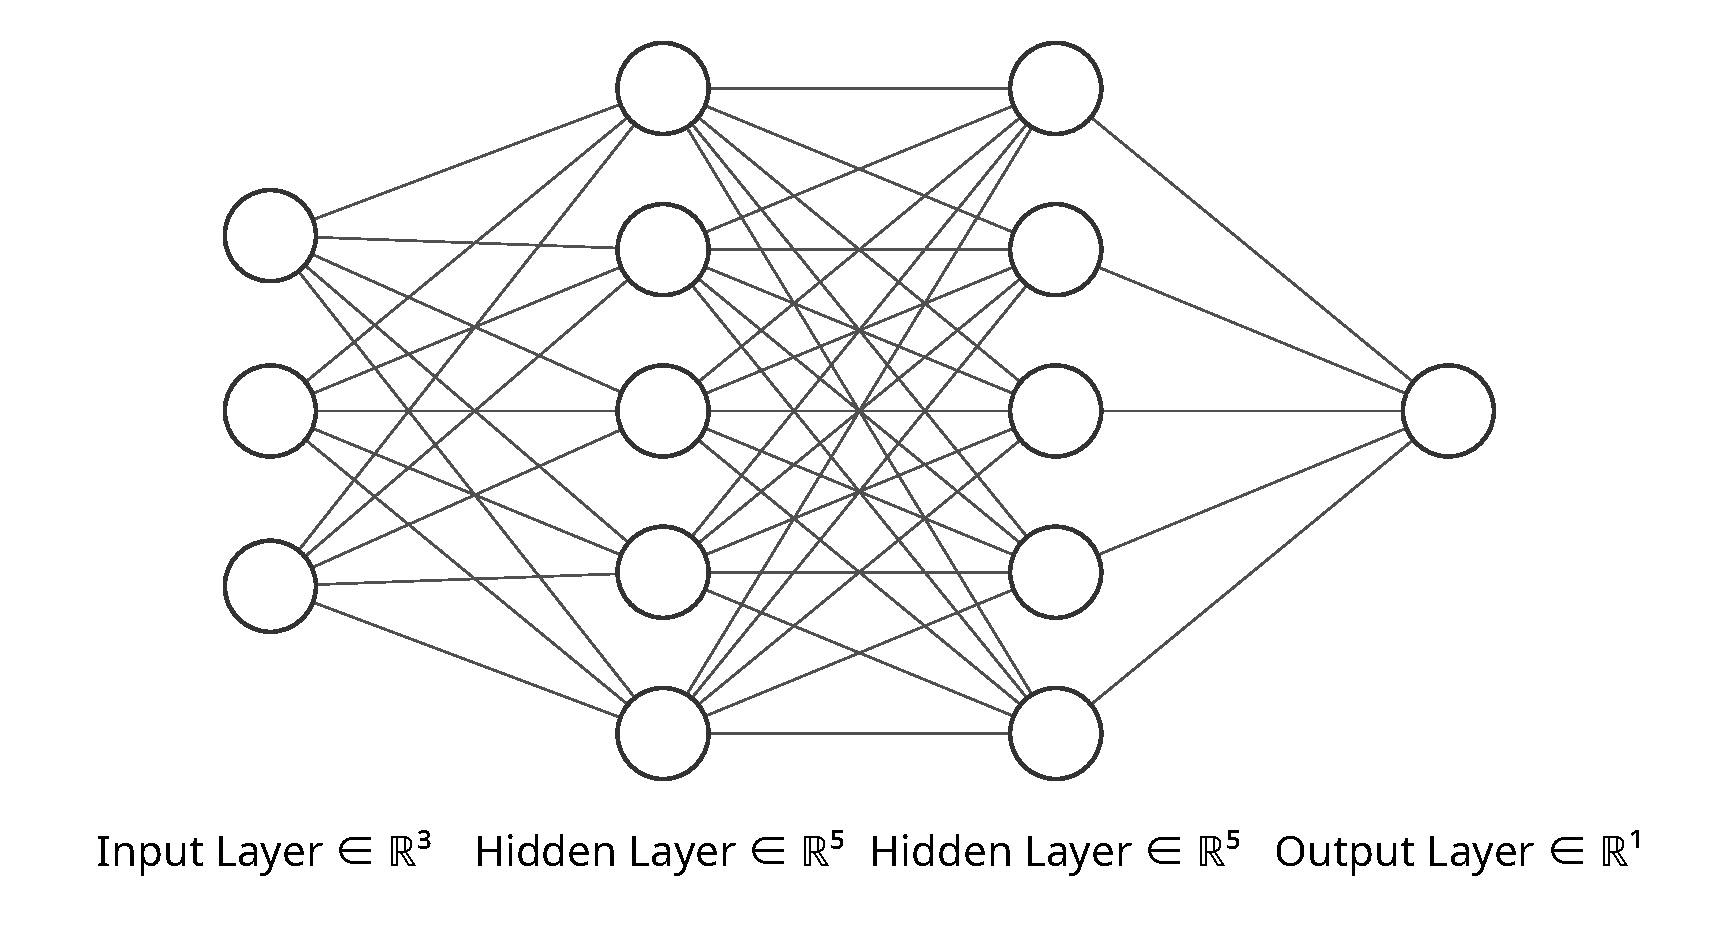
\includegraphics[width=\linewidth]{ml/nn_example.pdf}
        \caption{An example of a densely-connected
        neural network with two hidden layers.
        Each node on this image represents
        a neuron and the connections between then
        represents the inputs/outputs to neighbouring neurons.}
        \label{fig:nn_example}
    \end{figure}

    The depth of a neural network
    is generally denoted by the number of hidden layers,
    or alternatively, the number of activation functions
    between the input and output layers. Similarly,
    the width of a neural network is generally referring
    to the number of nodes in the hidden layers.

    The output of a densely-connected neural network can
    be formulated by repeatedly applying Eq. (\ref{eqn:neuron})
    to give
    \begin{equation}\label{eqn:nn_output}
        % f(\mathbf{x}; \theta) = \boldsymbol{\phi}^{(n)}(\ldots \boldsymbol{\phi}^{(2)}(\; \boldsymbol{\phi}^{(1)}(\mathbf{x}; \theta^{(1)})\; ; \theta^{(2)}) \; ; \theta^{(n)}) \, ,
        f(\mathbf{x}; \theta) = \boldsymbol{\phi}^{(n)}_{\theta}(\; \ldots \boldsymbol{\phi}^{(2)}_{\theta}\; (\boldsymbol{\phi}^{(1)}_{\theta}(\mathbf{x}) ) \; ) \, ,
    \end{equation}
    where $\boldsymbol{\phi}^{(n)}_{\theta}$
    denotes the outputs and parameters of layer $n$,
    where the output layer is included in this notation.
    By chaining together activation functions, and especially
    non-linear activation functions, neural networks
    become good function approximators
    \begin{equation}\label{eqn:nn_approx}
        f(\mathbf{x}; \theta) \approx g(\mathbf{x}) \, .
    \end{equation}
    The universal approximation theorem states that neural networks are
    able to represent any continuous function, $g(\mathbf{x})$,
    with one hidden layer and a finite number of neurons \cite{HORNIK1991251}.
    However, it is very difficult to achieve this due to
    practical constraints such as limited data and network size.
    It is much more common to link
    together a larger number of hidden layers, leading
    to deep neural networks since better learning algorithms
    have been found for this case \cite{lu2017expressive}.
    
\subsection{Loss functions and optimisation of parameters}
    To summarise so far, neural networks are a vast network
    of connected nodes with a large number of parameters that
    can be tuned for the problem at hand.
    The task of optimising the parameters is the main challenge
    in training a neural network and is a key area of research.

    In order to quantify the performance of a network for
    a given task it is useful to define a loss function.
    For regression tasks, such as approximating a function,
    a commonly used loss function is the mean squared error
    \begin{equation}\label{eqn:MSE}
        L_{\mathrm{MSE}} = \dfrac{1}{N} \sum_{i=1}^{N} (g(\mathbf{x}_{i}) - y(\mathbf{x}_{i}; \theta))^{2} \, ,
    \end{equation}
    where $g(\mathbf{x}_{i})$ and $f(\mathbf{x}_{i}; \theta)$
    are samples from the target distribution, and model predictions
    for inputs, $\mathbf{x}_{i}$, belonging to a data set with $N$
    samples. The loss function
    encodes the discrepancy between the truth value
    and the model prediction. Therefore, the task of finding
    an acceptable set of parameters can be reframed as an optimisation
    of the loss function. It should be noted that minimisation of
    the loss function is simply a proxy for maximising neural network
    predictive accuracy. Due to the training and testing datasets being finite,
    the generalisation of the neural network is not guaranteed for the
    true underlying function from which the datasets are sampled
    from. This problem is generally referred to as overfitting.
    We will refer back to this problem in the context of
    fitting matrix elements in Section~\ref{sec:NN_ME}.

    Since neural networks are generally aimed at
    learning non-linear functions, the loss surface
    corresponding to Eq. (\ref{eqn:MSE}) is
    a function of many variables, and is likely highly
    non-convex with many local minima.
    The methods of choice for traversing these loss surfaces
    are all iterative gradient-based methods with modifications
    to improve convergence. Broadly speaking, the algorithms
    iteratively update the neural network parameters based on the
    gradient of the loss with respect to these parameters
    with some step size (or learning rate) $\eta$. The update
    rule is given by
    \begin{equation}\label{eqn:gradient_descent}
        \theta \gets \theta - \eta \cdot \nabla_{\theta} L(\mathbf{x}_{\mathrm{batch}}; \theta) \, ,
    \end{equation}
    where $\nabla_{\theta}L(\mathbf{x}_{\mathrm{batch}}; \theta)$ is the
    gradient of the loss with respect to the parameters of the
    model, averaged over the batch of inputs $\mathbf{x}_{\mathrm{batch}}$.
    The initial state of the parameters
    are usually distributed according to normal
    or uniform distributions \cite{pmlr-v9-glorot10a,he_initialiser}.
    This variation of gradient descent is referred to
    as mini-batch gradient descent because the gradient
    $\nabla_{\theta}L$ is averaged over a mini-batch of
    samples $\mathbf{x}_{\mathrm{batch}}$. Mini-batch gradient
    descent strikes a balance between stochastic gradient
    descent (estimating gradient with one sample at a time),
    and batch gradient descent (calculating gradient with
    respect to entire training set) by having an efficient
    estimation of the gradient that is accurate enough
    for practical applications. In modern machine learning
    libraries, the updating of weights in Eq. (\ref{eqn:gradient_descent})
    is carried out via matrix multiplications which are
    highly efficient on graphics-processing units (GPUs),
    and the gradients are computed numerically with the aid
    of automatic differentiation tools. For these reasons, deep
    neural networks have become much more widespread due
    to the ease of constructing and training them, as well
    as their good predictive performance for general problems.

    The basic gradient descent algorithm described above
    is the basis upon which many of the most widely
    adopted optimisers \cite{kiefer1952stochastic,hintonrmsprop,Kingma:2014vow}
    are based on. For an overview of these optimisers, see for instance
    Ref. \cite{Ruder:2016lil}.

    \subsection{Optimisation of hyperparameters}
    \label{sec:hyperparameters}
    Another set of parameters that need to be optimised
    are the model hyperparameters.
    Hyperparameters are parameters that are
    not explicitly trainable parameters of the model, instead they control
    the speed and quality of the training process.
    For instance, the learning rate in Eq. ({\ref{eqn:gradient_descent}}) is
    an important hyperparameter whose initial value has
    to be chosen carefully to observe a good rate of convergence.
    Some other examples would be
    the number of hidden layers, the choice of activation
    function, or the mini-batch size.

    The choice of hyperparameters is an important
    factor during the training process as a suboptimal set
    of hyperparameters can perform significantly worse
    than a more carefully chosen set. The process of tuning
    hyperparameters is often computationally expensive for two
    reasons. Firstly, the dimensionality of parameter space to
    choose from is large, meaning the number of samples required
    to effectively explore the parameter space grows rapidly --
    this is the so-called curse of dimensionality.
    Secondly, there is no exact a priori way to evaluate the
    final performance of a neural network given a set of
    hyperparameters, meaning training has to take place for
    some steps before the final model performance can be estimated.
    
    Some of the simplest methods of hyperparameter optimisation
    are grid search and random search. Grid search is simply
    an exhaustive scan of parameters systematically sampled
    in a grid-like fashion, whereas random search replaces
    this systematic sampling with random sampling. Whilst
    these methods are quick to implement, the number of trials
    to land on a good set of hyperparameters could potentially
    be very large. Methods which aim to reduce the number
    of trials have been proposed in the literature, see Ref.
    \cite{Yu2020HyperParameterOA} for a review.
    Below we discuss two paradigms of hyperparameter optimisation
    that aim to reduce number of trials when doing hyperparameter searches.

    Bayesian optimisation methods have been explored
    to carry out hyperparameter optimisation \cite{bergstra2013making,bergstra2015hyperopt}.
    The method begins with the construction of a 
    Bayesian probabilistic model. This model is a mapping
    from hyperparameter sets to the performance
    of a neural network, as evaluated by a loss function. 
    This Bayesian model collects evidence
    through successive trainings of the neural network,
    and so iteratively becomes more informed on the hyperparameter
    space. By selecting promising hyperparameter
    sets based on the successively updated model, the exploration of
    hyperparameter space is much more efficient.

    Another group of methods are based on the principle
    that the first few epochs of training are indicative
    of the final model performance \cite{pmlr-v28-bubeck13}. This in combination
    with a fixed time budget gives rise to multi-armed
    bandit strategies \cite{jamieson2016non,li2017hyperband}
    that allocate more budget to better
    performing models whilst simultaneously dropping poorly
    performing models. By iterating this procedure only the 
    best performing models remain. Recently, there have
    been proposals of combining Bayesian optimisation and
    the bandit-based approaches \cite{falkner2018bohb}.
    
    In practice, the area of hyperparameter optimisation
    is still extremely computationally expensive even with
    the more advanced methods outlined above. Given a sensible set of hyperparameters,
    one has to balance the additional time spent tuning with the
    relatively incremental improvements in performance. For this reason,
    the hyperparameter tuning in novel machine learning experiments
    in high energy physics is not of paramount importance.
    Instead more focus is spent on the model building itself, as
    more sophisticated models represent a more substantial increase
    in performance.

\section{Neural networks as matrix element surrogate models}\label{sec:NN_ME}
    Motivated by the ability of neural networks to
    model non-linear functions, as well as the rise
    in GPU usage in high energy physics, it seems
    natural to leverage neural networks to build surrogate
    models for matrix elements. There are multiple advantages
    to this: the time taken to evaluate matrix elements remains
    a bottleneck in event generation, and so building a
    fast surrogate model would accelerate this process.
    Once a fast and accurate surrogate model has been
    built, it can supplement traditional matrix
    element generators to increase statistical power of the sample
    by evaluating on many more phase-space points efficiently. This
    requires the accumulated error in the surrogate model
    predictions to be lower than the statistical error in the
    integration of matrix elements, which is a key motivation
    for building an accurate surrogate model.

    Related to the problem of modelling matrix elements, in recent
    years there has been work in applying machine learning
    methods to learn: event weights \cite{Danziger:2021eeg},
    cross-sections \cite{Otten:2018kum,Buckley:2020bxg},
    analytic expressions of squared amplitudes \cite{Alnuqaydan:2022ncd},
    contour deformations for multi-loop integrals \cite{Winterhalder:2021ngy},
    and simplifying polylogarithms \cite{Dersy:2022bym}.

    The task of building a surrogate
    model for matrix elements is in principle straightforward.
    The dataset usually consists of phase-space kinematics
    in the form of four-momenta and the targets are the
    corresponding matrix elements for the process of interest,
    at the desired order in perturbation theory. As already
    discussed in Sections~\ref{sec:MC_integration} and \ref{sec:me_generators},
    phase-space samplers and matrix element generators are
    now widely available so the acquisition of data is only
    limited by available computing time. Even then, this is a bottleneck only
    for the most expensive of processes as generation
    of data is trivial to parallelise. In the ideal case, the
    surrogate model would be faster than the matrix
    element generators, and sufficiently accurate. Neural
    network predictions are fast by virtue of them being
    simple matrix multiplications, and because they are predicted
    in batches, vectorisation is automatic\footnote{Event generators currently generate events one at a time, however, neural network predictions are still highly performant for single predictions.}.
    Therefore the difficulty
    in building a good surrogate model is in controlling
    the accuracy.

    The complication in accurately emulating matrix elements
    on a per-point basis arises due to the infrared divergent behaviour,
    as discussed in Section~\ref{sec:IR_divergences}, which occurs
    in corners of the phase-space
    (UV divergences have been removed via renormalisation).
    Outside of these soft and collinear limits, the matrix element
    is a well-behaved function that varies smoothly with phase-space.
    However, once these infrared regions are approached, small changes in the
    kinematics can lead to very large changes in the matrix
    element. This rapid response in the target
    function makes it difficult to accurately model the
    non-divergent regions simultaneously with the divergent
    regions, due to the disparity in scales. This problem
    becomes more apparent for higher multiplicity final-states
    as there are more regions in phase-space for which
    the matrix element diverges.

    Emulation of matrix elements directly have been
    carried out in recent years in various projects.
    Bishara and Montull showed \cite{Bishara:2019iwh} that it was possible to
    build a boosted decision tree model to reproduce
    the matrix elements of the loop induced process $gg \rightarrow ZZ$ with good accuracy --
    below 0.1\% errors for fully differential distributions.
    However, for this $2 \rightarrow 2$ process it was already demonstrated
    that training a single model on the entire phase-space sampled
    was suboptimal compared to training a number of regressors
    on subdomains of the phase-space.

    This trend was observed in a future work by Aylett-Bullock
    and Badger \cite{Badger:2020uow} where the authors emulated tree-level
    matrix elements and NLO QCD K-factors for $e^{+}e^{-} \rightarrow q \bar{q}$ +
    up to 3 gluons. With a higher final-state multiplicity, controlling
    the infrared divergences became a crucial challenge.
    Their approach was to first partition phase-space
    into divergent and non-divergent regions, then subsequently
    weight the divergent regions further according to partition functions
    based on FKS subtraction.
    In each weighted partition, the authors trained a separate neural network,
    meaning that their model was an ensemble of neural networks.
    The performance of this method was shown to be an improvement
    over a single neural network trained on the unpartitioned phase-space,
    with good agreement in histogrammed distributions. However,
    the per-point agreement was lacking.

    This FKS partitioning method was applied in Ref. \cite{Aylett-Bullock:2021hmo}
    for diphoton plus jet production, where the authors presented a
    use case of the emulator with a novel interface to the {\Sherpa} event generator.
    This work was revisited in Ref. \cite{Badger:2022hwf},
    where particular attention was paid to quantifying the uncertainty associated
    with the neural network prediction. This uncertainty was
    modelled with a Bayesian neural network which enabled
    the boosted training on regions of phase-space that were
    lacking in accuracy. Additionally, the authors showed
    that accuracy was improved with a more careful
    preprocessing of the training data compared to
    the previous treatment.
    However, both of these works showed that increasing
    multiplicity from $2 \rightarrow 3$ to $2 \rightarrow 4$
    represented a large decrease in accuracy.

    To summarise, the current state of matrix element
    emulation has to trade-off higher multiplicity processes
    with accuracy. The research in this thesis attempts to
    tackle both of these problems by exploiting the factorisation
    property of matrix elements (Sections \ref{sec:me_factorisation},
    \ref{sec:CO_factorisation}, and \ref{sec:OL_factorisation}),
    to build into the emulator the universal singular functions
    that describe the matrix elements in the soft and collinear limits
    (Sections \ref{sec:CS_dipoles} and \ref{sec:antenna_functions}).
    Since this method relies on the factorisation of matrix
    elements, we collectively refer to these family of models
    as factorisation-aware models.
    In Chapter~\ref{chapter:fame1}, we show that by forming an ansatz
    out of a linear combination of Catani-Seymour dipoles with
    fitted coefficients, tree-level
    matrix elements for $e^{+}e^{-} \rightarrow q \bar{q}$ + up to 3 gluons
    can be emulated accurately to well below 1\% per-point accuracy,
    even for the highest multiplicity. Extending this study
    to the one-loop level is done in Chapter~\ref{chapter:fame2},
    where antenna functions replace Catani-Seymour dipoles as
    the ingredients in the ansatz. Accuracy was observed to be of the
    order 1\% for the 5 parton case, with good scaling
    to higher multiplicities.

    The question of uncertainty of the neural network
    prediction is important as it directly contributes to the total
    theoretical uncertainty. An alternative to quantifying
    the uncertainty of the neural network prediction is to
    use the prediction in an intermediary step of a full
    calculation, where the final prediction comes from the
    accustomed matrix element providers. This was explored in
    Ref. \cite{Danziger:2021eeg},
    where it was shown that with a surrogate model of the event
    weight it was possible to use a double unweighting
    algorithm to increase the rate of event unweighting.
    In Chapter~\ref{chapter:fame3} we examine replacing
    the original emulator in that work with a factorisation-aware
    model to study the potential gain factors with a more
    accurate model. As previously mentioned, a consequence of
    this two-stage unweighting
    algorithm is that the exact event weight has to be evaluated
    at some point, meaning the uncertainty of the surrogate
    model is practically irrelevant.
\end{document}